\chapter{Irodalmi áttekintés}
\section{Ipari ütemezési feladatok}
Az ipari folyamatokat gyártásnak nevezzük, amely során az elkészítendő termék létrehozása, megvalósítása a feladat. Ehhez szükség van arra, hogy megfelelően vegyük igénybe a rendelkezésre álló erőforrásokat, amelyeket berendezéseknek, unitnak nevezünk a gyártási feladtok során. A folyamat során fellépő feladatokra a taszk elnevezés is használható. Minden ütemezési feladat rendelkezik végrehajtási idővel, ami megmutatja mekkora időtartam alatt valósítható meg. Ezenfelül lehet még a feladatoknak olyan időkorlátja, ami alatt kötelező elvégezni a feladatot, ezt időhorizontnak, time horizontnak hívunk. A problémák kimenetelük szerint lehetnek megvalósíthatatlan (infeasible) és megvalósítható (feasible) feladatok. Ha egy korlátozásnak sem felel meg az adott probléma akkor infeasible, egyéb esetekben pedig már megvalósítható lesz.

Az ipari folyamatokat többféleképpen lehet csoportosítani. Egy fajta az, amelyben folyamatos és szakaszos üzemű rendszerek csoportjára bontjuk őket. Az első típusban az anyag folyamatosan kerül a rendszerbe, a másodikban pedig ez a folyamat lépésekben valósul meg. A munkám az utóbbi típusba tartozó feladatokra koncentrál. Másik lehetséges felosztás az, amikor online, offline, és semi-offline kategóriákba vannak a feladatok besorolva. Az offline esetben minden szükséges bemeneti adat rendelkezésre áll az optimalizálás idejében. Az online ezzel szemben úgy működik, hogy előbb kell döntéseket meghozni, minthogy adott paraméterekhez tartozó értékekre fény derülne. A semi-offline a kettő közé sorolható. Bizonyos információk, adatok már rendelkezésre állnak, mások viszont nem. Egy harmadik besorolási lehetőség, hogy megkülönböztetünk sztochaikus és determinisztikus feladatokat. Sztochaikus esetekben a paraméterek már futás közben kapnak értéket. Ezzel szemben a determinisztikus feladatok értékei előre meg vannak határozva és beállítva.

Az ütemezési feladatok modelljét receptnek nevezzük. Egy termék receptje tartalmazza az adott recept által előállítható termék elkészítéséhez szükséges információkat\cite{Hegyhati}. Egy receptet következő elemek együtt alkotják meg:
\begin{itemize}
  \item Termékek listája
  \item Taszkok listája, amelyek adott sorrendben történő elvégzése szükséges a termékek előállításához
  \item Taszkok egymás közötti sorrendisége, amely megmutatja a taszkok sorrendjét
  \item Rendelkezésre álló berendezések
  \item A lehetséges taszk-berendezés párok feldolgozási ideje
\end{itemize}
A recepteket a feladatok precedenciájuk szerint következő csoportokba lehet besorolni. A felsorolás a legegyszerűbbtől halad az általánosabb felé. Ezen kívül minden osztály a következőnek egy speciális esete.
\begin{itemize}
	\item \textbf{Single Stage:} Egy lépésben állítható elő minden egyes termék.
	\item \textbf{Simple Multiproduct:} Minden terméket meghatározott számú fázison, szakaszon keresztül lehet elkészíteni. Előzővel szemben itt már nem csak egy lépésben lehetséges.
	\item \textbf{General Multiproduct:} Előzővel összehasonlítva a különbség, hogy ennél lehetséges lépések kihagyása.
	\item \textbf{Multipurpose:} A termékek gyártásának lépéseit nem lehet egy balról jobbra tartó vonal mentén véghezvinni. A szakaszok száma és iránya tetszőleges, sőt egy szakasz többször is ismétlődhet ugyanabban a gyártásban.
	\item \textbf{Precedential:} A gyártásban résztvevő taszkok nincsenek hozzárendelve a szakaszokhoz. Egy termék gyártás nem szükségszerűen lineáris, lehetnek elágazások, kör azonban nem megengedett. Minden taszk előfeltételét be kell fejezni mielőtt az adott lépés megkezdődik. 
	\item \textbf{General Network:} A legáltalánosabb recept, ahol a taszkok a bemenetük és a kimenetük által adottak. Ennél az esetén kör is lehetséges.
\end{itemize}
Néhány előbb említett feladattípus szemléltetése látható a~\ref{receptek} ábrán. A receptek jobb oldalán lévő kör jelenti a terméket, a többi pedig a taszkokat.
\begin{figure}[H]	
\begin{center}
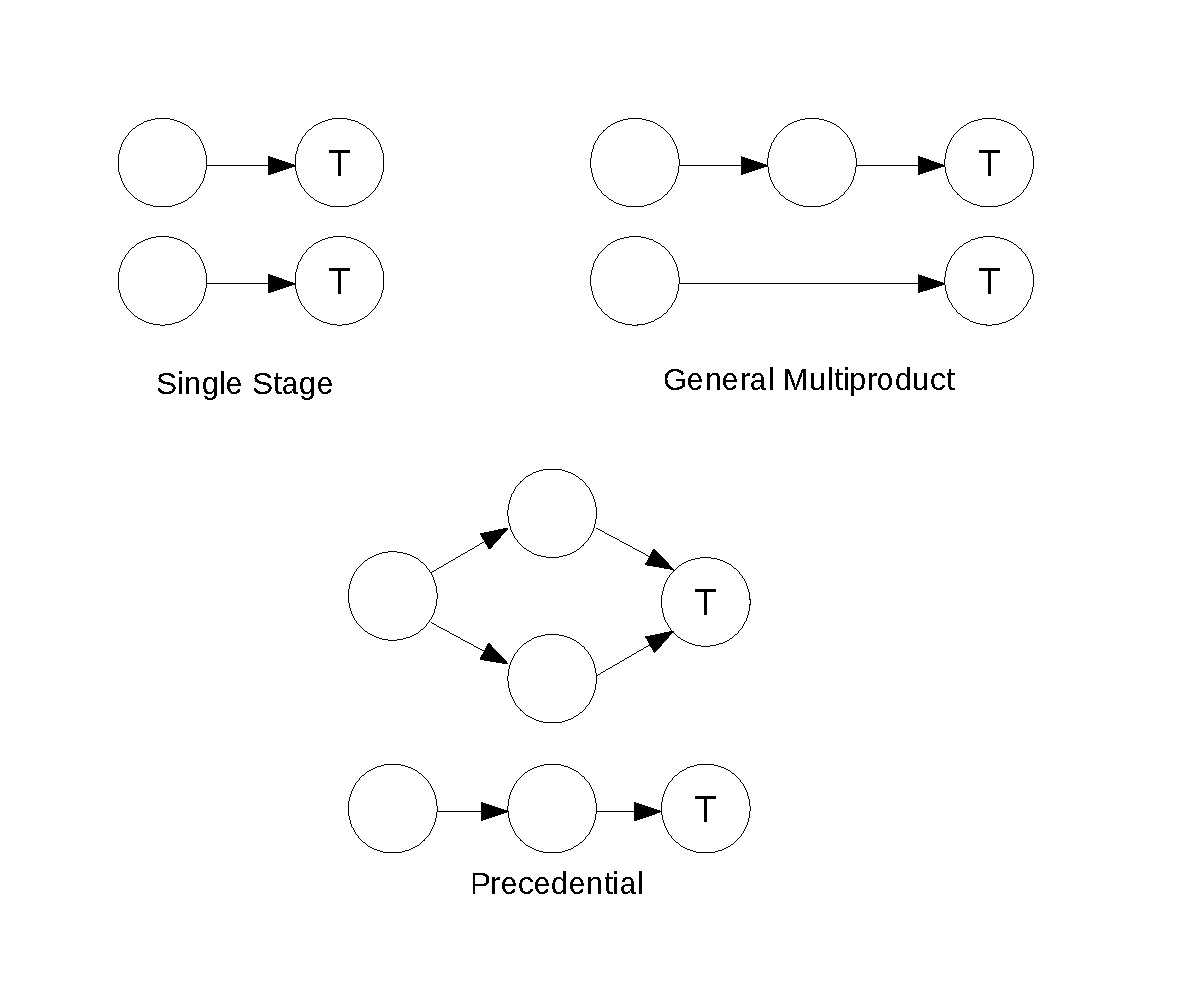
\includegraphics[scale=0.7]{receptek}
\caption{Különböző receptek szemléltetése}
\label{receptek}
\end{center}
\end{figure}
\newpage
A vegyipari, gyártási ütemezési feladatoknál nagy szerepet játszik a tárolási irányelv. A tárolási irányelvek azt mutatják meg, hogy két egymást követő feladatok között az elkészített köztes termékeket, hogyan kell raktározni, tárolni, illetve ez mennyi ideig lehetséges. A tárolási stratégiák csoportosításra többféle lehetőség van. Egyik ezek közül, amikor az adott létesítmény infrastrukturális képességei korlátozzák az anyag mennyiségét és minőségét.
\begin{itemize}
	\item \textbf{UIS - Unlimited Intermediate Storage}
	\item \textbf{FIS - Finite Intermediate Storage}
	\item \textbf{NIS - No Intermediate Storage}
\end{itemize}
Az UIS eset a legegyszerűbb. Ebben az esetben van lehetőség a köztes anyagok bármely mértékű tárolására. FIS esetben van lehetőség a tárolása, de csak korlátozott mennyiségben. A NIS esetében nincs külön tárolásra alkalmas egység, de az megoldható, hogy amíg a következő feldolgozó egységhez kerül, addig az előző helyen várakozzon.

Második fajta csoportosítási lehetősége, amikor az idő ad korlátot.
\begin{itemize}
	\item \textbf{UW - Unlimited Wait}
	\item \textbf{LW - Limited Wait}
	\item \textbf{ZW - Zero Wait}	
\end{itemize}
ZW esetben nincs lehetőség a köztes anyag tárolására, azaz ha a berendezés befejezte a munkát, akkor azonnal folytatni kell a gyártást. AZ LW esetben van egy idő, amíg a köztes termék várakozhat. Azonban, ha ez a rendelkezésre álló idő elfogy, akkor muszáj folytatni a gyártás folyamatát. Az UW eset a legegyszerűbb mind közül. Ha a köztes anyag tulajdonságai lehetőséget biztosítanak, akkor a tárolási idő nincs korlátozva, bármennyi ideig lehetőség van a tárolásra, raktározásra.
\newpage
\section{Megoldó módszerek}
Az ütemezési feladatok megoldására számos megoldó módszer létezik. Ezek közül a legismertebbek, és legszélesebb körben elterjedt módszerek kerülnek bemutatásra a dolgozatom következő pontjaiban.
\subsection{MILP modellek}
A legtöbb ütemezési probléma modelljében vegyesen fordulnak elő folytonos és egész változók. Ilyen esetekben beszélünk vegyes egészértékű lineáris programozásról, azaz \textbf{M}ixed \textbf{I}nteger \textbf{L}inear \textbf{P}rogramming. Több altípus létezik:
\begin{itemize}
  \item[] \textbf{Időfelosztásos modellek - Time discretization based:} A módszer időpontokat és időréseket határoz meg. Ezek jelentek meg legkorábban kronológiailag \cite{kondili}. Az időrésen és az időponton alapuló megközelítések \cite{susarla} sok hasonlóságot mutatnak, mivel egy időintervallumtól egy másikig terjedő időintervallumot tekinthetünk időrésnek. Ellenkező irányból nézve pedig egy időrés kezdő időpontját tekinthetjük egy időpontnak.  
  
  Minden időpontban bináris változók vannak hozzárendelve aszerint, hogy az adott időpillanatban kezdődik a feladat végrehajtása vagy nem. A bináris változók száma arányos lesz az időpontok számával. A szándék mindig megvolt olyan módszer kifejlesztésére, amelyben a szükséges időpontok száma minél kisebb legyen amellett, hogy megtalálja az optimális megoldást. 
  
  \item[] \textbf{Precedencia alapú modellek - Precedence based:} Ezeknél a módszereknél, szemben az időfelosztásos módszerekkel, nincs szükség az időhorizont diszkretizációjára, nem használnak ismeretlen paramétert a modellben. Általánosságban jobb számítási eredményeket nyújtanak az általuk kezelt problémákra, azonban ez a készlet sokkal kisebb, mint az időfelosztásos modellekhez tartozó kollekció. Alapvetően a multiproduct és multipurpose receptek esetében használható megfelelően, de kibővíthető, hogy a sokkal általánosabb precedential receptek is megoldhatók legyenek. 
  
  Ez a módszer kettő darab bináris változó használ. Az első $Y_{i,j}$, aminek az értéke abban az esetben lesz 1, ha $i$ feladatot $j$ berendezés végzi el. A második változó: $X_{i,j,i'}$. Értéke akkor lesz 1, ha ugyan az a berendezés végzi el az $i$ és $i'$ taszkot, méghozzá úgy, hogy előbb az $i$-t teljesíti. 
\end{itemize}
\subsection{Analízis alapú eszközök}
Az automatákat és Petri hálókat széles körben alkalmazzák diszkrét eseményrendszerek modellezésére \cite{cassandras}. Számos kísérletet tettek ezen eszközök modellezési teljesítményének kiterjesztésére annak érdekében, hogy batch folyamatok ütemezésére is alkalmassá tegyék. A meglévő modelleket időzítéssel egészítették ki, így jöttek létre, a Timed Place Petri Nets (TPPN) and Timed Priced Automata (TPA) módszerek, amelyek Branch and Bound algoritmus használnak azért, hogy a legelőnyösebb megoldást megtalálják. Ezen módszereknek a hatékonysága elmarad a MILP és az S-gráf modell hatékonyságától is.
\begin{itemize}
	\item[] \textbf{Időzített automaták:} Ezekben a megközelítésekben a recepteket és a berendezéseket külön modellezik, és a rendszer modellje ezeknek a párhuzamos összetételével jön létre. A bonyolultságos az jelenti, hogy az órák állapota végtelen lehet, és emiatt a rendszer állapotterülete is az lehet.
	\item[] \textbf{Időzített Petri háló:} Az alap ilyen módszereknél, hogy az átvitel jele késleltetés alapján jön létre. Többen is foglalkoztak a témával, például Ghaeli \cite{ghaeli}, aki batch folyamatok ütemezésével foglalkozott.
\end{itemize}

\subsection{S-gráf módszertan}
Az S-gráf keretrendszer volt az első olyan módszer, amely publikált gráf elméleten alapult, valamint szakaszos gyártórendszerek ütemezési problémák megoldására szolgált.\cite{combtech} Ez a keretrendszer egy irányított gráf modellből, az S-gráfból, és a hozzá tartozó algoritmusokból áll. \cite{combframe} Az S-gráf egy speciális irányított gráf, ami ütemezési problémák számára. Nemcsak a recept vizualizációja, hanem egyben matematikai modell is. A keretrendszerben az S-gráf reprezentálja a recepteket, a részleges és a teljes ütemterveket is. Ezekben a gráfokban a termékeket és a feladatokat csúcsok jelölik, amelyeket csomópontoknak (node) nevezünk. Ha két feladat között összeköttetés van, akkor ezt a gráfon lévő, feladatokat reprezentáló csomópontok között lévő nyíl mutatja. Ütemezési döntés nélküli S-gráfot \textbf{Recept gráfnak} nevezzük. Erre példa a~\ref{receptGraf} ábrán\cite{Hegyhati} látható. 

A jobb oldalon látható három, nagybetűvel jelölt csomópont felel meg a termékeknek, a maradék kilenc pedig a részfeladatokat jelenti. Ezt a kilenc részfeladatot el kell végezni a termékek előállításának érdekében. Az élek (nyilak) a csomópontok közti függőséget mutatják meg. Ezeket \textbf{Recept éleknek} nevezzük. Kétfajta függőséget tudunk megkülönböztetni:
\begin{itemize}
  \item Két részfeladat között van él. Ebben az esetben az egyik készíti el a másiknak a bemenetét.
  \item Egy termék és egy részfeladat között szerepel él. Ilyenkor a részfeladat készíti el a terméket.
\end{itemize}
A nyilakon látható súlyok a részfeladat végrehajtásához szükséges időt mutatják meg. Ha egy részfeladatot több berendezés is képes elvégezni, akkor az előbb említett súly mindig a legkisebb előállítási idő lesz.
\begin{figure}[H]	
\begin{center}
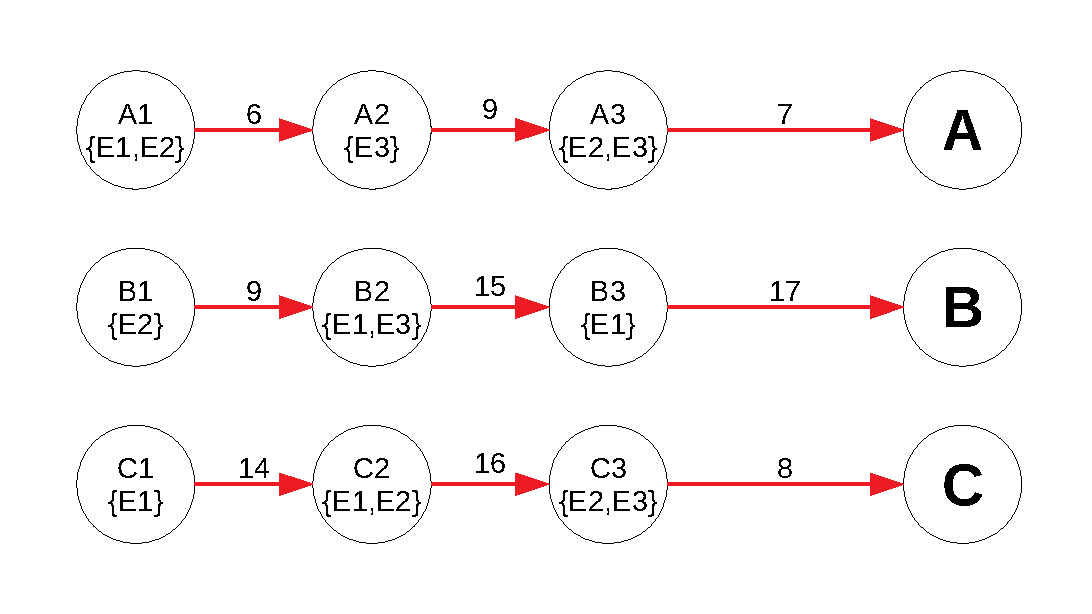
\includegraphics[scale=0.7]{receptGraf}
\caption{A recept gráf szemléltetése}
\label{receptGraf}
\end{center}
\end{figure}
Minden S-gráf-hoz kapcsolódó algoritmus kiegészíti ezeket a gráfokat az úgynevezett \textbf{ütemezési élekkel}, amelyek az ütemezési döntést testesítik meg. Ezekkel az élekkel kiegészített gráfoknak a neve \textbf{Ütemezési gráf}. Példa a~\ref{utemezesiGraf} ábrán nézhető meg. Az ábrán sötétkékkel jelölt nyilak az ütemezési élek. Az ütemezési élek súlya alapértelmezetten nulla, ha a probléma nem tartalmaz szállítási, vagy tisztítási időt. A részfeladatok csomópontjain már nem a lehetséges berendezések halmaza látható, hanem egy konkrét kiválasztott berendezés, az ütemezési döntésnek megfelelően. 
\begin{figure}[H]
\begin{center}
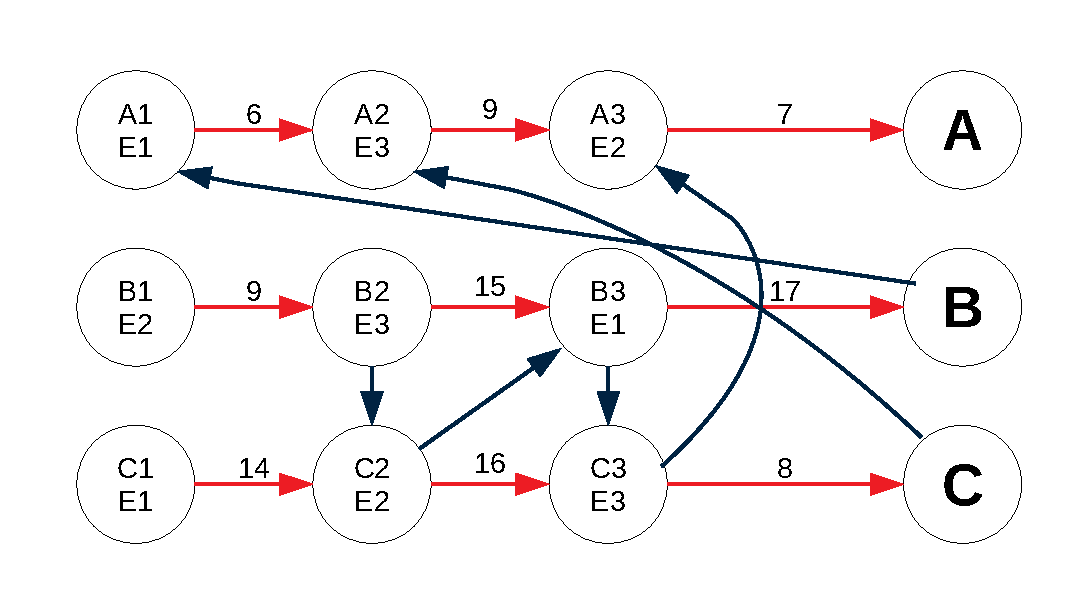
\includegraphics[scale=0.7]{utemezesiGraf}
\caption{Az ütemezési gráf szemléltetése}
\label{utemezesiGraf}
\end{center}
\end{figure}
Ugyanahhoz a berendezéshez rendelt részfeladatok végrehajtási sorrendje könnyedén leolvasható a gráfról. A~\ref{utemezesiGraf2} ábrán látható példában az E2-es berendezés által elvégzett részfeladatok sorrendje B1 -\textgreater  C2 -\textgreater  A3. Ahhoz, hogy a berendezés el tudjon végezni egy adott részfeladatot nem elég, hogy az általa végzett előző részfeladatot befejezze, hanem szükség van még ezen kívül arra, hogy a soron következő részfeladathoz szükséges összes részfeladat elkészüljön. Csak ezeket követően tudja megkezdeni az adott részfeladat végrehajtását. Példa: C2-es részfeladat végrehajtásához szükséges, hogy az E2-es berendezés befejezze a B1-es részfeladatot, valamint az is, hogy a C1-es részfeladatot elkészítse az E1-es berendezés.
\begin{figure}[H]
\begin{center}
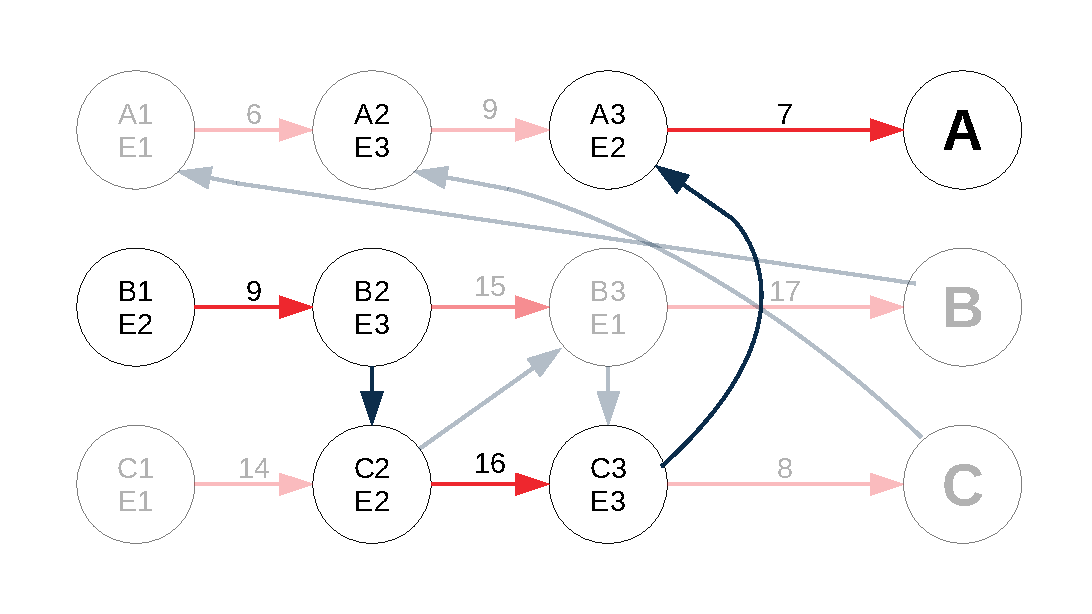
\includegraphics[scale=0.7]{utemezesiGraf2}
\caption{E2-es berendezés által elvégzett részfeladatok}
\label{utemezesiGraf2}
\end{center}
\end{figure}
Gyakran használt mód az ütemezési feladatok ábrázolására a Gantt-diagram\cite{ganttwwf}\cite{ganttofw}. Ezeken a diagramokon a függőleges tengelyen a berendezések, míg a vízszintes tengelyen a pedig az idő szerepel. Az ábrán látható erőforrások szemléltetik az erőforrások elfoglaltságát. Egy Gantt diagram látható a~\ref{GanttDiagram} ábrán.
\begin{figure}[H]
\begin{center}
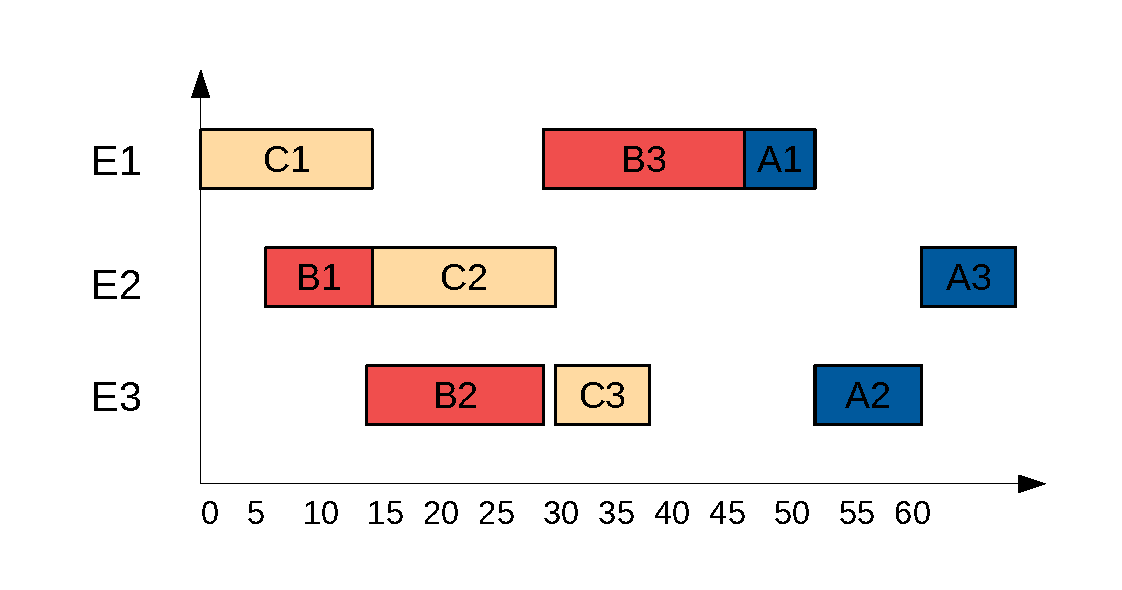
\includegraphics[scale=0.7]{GanttDiagram}
\caption{Egy ütemezés Gantt diagramon való megjelenítése}
\label{GanttDiagram}
\end{center}
\end{figure}

\subsection{A makespan minimalizálás algoritmusa}
Az algoritmus \ref{makespanKod} első lépésben inicializálja a $makespan^{cb}$ értékét végtelennel, majd beállítja a $S$ halmazt, amelyben az ütemezés során a nyitott részproblémák szerepelnek. Kezdetben csak a gyökér probléma szerepel benne, vagyis egy recept gráf bármilyen hozzárendelés nélkül. A \textbf{recipe} függvény visszaadja a $G(N,A_1,A_2,w)$ által jelzett probléma recept gráfját, ahol
\begin{itemize}
  \item[] $N$: taszkokat és termékeket reprezentáló csomópontok halmaza	
  \item[] $A_1$: a recept élek halmaza
  \item[] $A_2$: ütemezési élek halmaza, ebben a pillanatban még üres
  \item[] $w_{i,i'}$: recept élek súlya, ami az $i$ taszk minimális feldolgozási ideje .
\end{itemize}

Az iteráció minden lépésében a \textbf{select\_remove} függvénnyel egy tetszőleges részprobléma kerül kiválasztásra, majd az $s$-ből eltávolításra. Ennek a függvénynek a viselkedése a különböző megvalósításokban más és más lehet, ami más keresési stratégiát eredményez.

Az iteráció elején kiértékelődik, hogy a részprobléma képes-e optimális megoldást nyújtani, vagy sem. Ez a \textbf{bound} függvénnyel történik. A leggyakrabban a leghosszabb út keresésével vizsgálja meg a részproblémát \textbf{bound} függvény, de lehetséges LP alapú modellek használata is. Ha a korlát nem kisebb, mint az eddig megtalált legjobb eredmény, akkor az iteráció véget ér, és a következő részprobléma kerül kiválasztásra, amennyiben létezik.

Ha viszont kisebb a korlát, akkor ellenőrzi az algoritmus azt, hogy az összes taszk már ütemezett-e, azaz a részprobléma teljesen ütemezett. Ha így van a legjobb megoldás frissítésre kerül. Ha még szükséges további ütemezés, akkor a  \textbf{select} függvény kiválaszt egy rendelkezésre álló berendezést a $J'$ halmazból. A kiválasztott $j$ berendezéshez az algoritmus hozzárendeli az összes lehetséges taszkot. Ezek kapnak egy másolatot az aktuális S-gráfról. Ezt kibővíti az új hozzárendelés alapján az ütemezési élekkel. Végezetül pedig az új részproblémát hozzáadja az $S$ halmazhoz. Ha ez az $S$ halmaz üres lesz, akkor a $G^{cb}$ és a hozzárendelések leírják az optimális megoldást, és ha legalább egy megvalósítható akkor az algoritmus visszatér ezzel az értékkel. Ellenkező esetben nem ad vissza semmit.

\begin{figure}[H]
\begin{center}
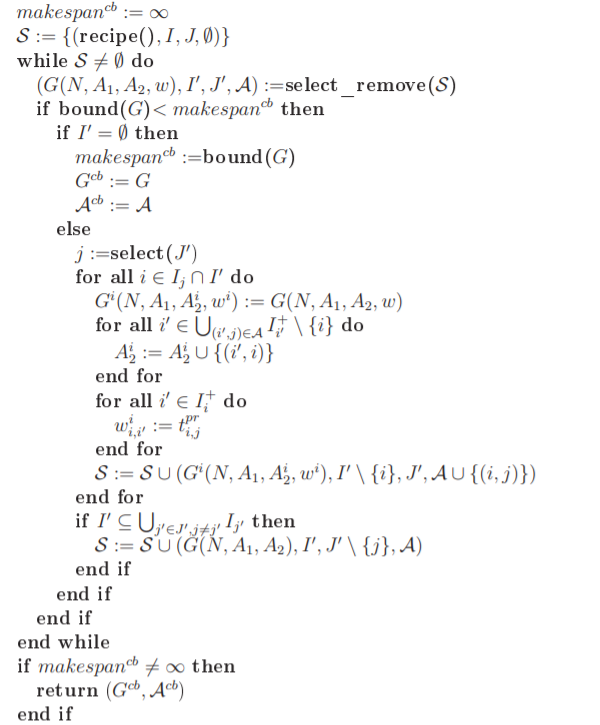
\includegraphics[scale=0.8]{makespanKod}
\caption{A makespan minimalizáló algoritmus pszeudó kódja\cite{Hegyhati}}
\label{makespanKod}
\end{center}
\end{figure}

\section{Throughput vagy profitmaximalizálás}
Eredetileg az S-gráf keretrendszer makespan minimalizációs problémák megoldására lett létrehozva. Azonban a későbbiekben bővítésre került, így ezután throughput, profitmaximalizációs problémák megoldására is lehet alkalmazni. Az alapötlet Majozi and Friedler \cite{majozifriedler}, valamint Holczinger \cite{holczinger} nevéhez fűződik.
\begin{figure}[H]
\begin{center}
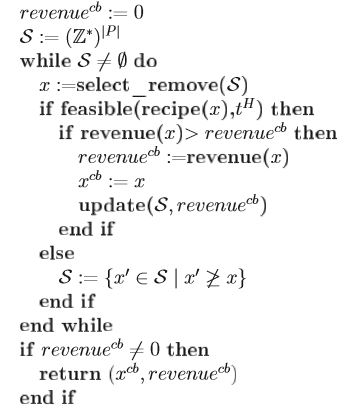
\includegraphics[scale=0.8]{throughput_alg}
\caption{A jövedelem maximalizáló algoritmus pszeudó kódja \cite{Hegyhati}}
\label{throughput_alg}
\end{center}
\end{figure}
Az algoritmus először inicializálja S halmazt, minden lehetséges batch számmal, a termékekre vonatkozóan. Fontos kiemelni, hogy ebben az esetben minden terméknél a batch méret rögzített. Ezt követően minden iteráció során az előbb említett halmazból kiválasztásra kerül egy konfiguráció a \textbf{select\textunderscore remove} függvény segítségével. Ezután kerül feasibiliy tesztelésre, amely során eldől, hogy a megadott időhorizont alatt megvalósítható vagy sem. Ha megvalósítható és nagyobb jövedelmet biztosít, akkor a jelenlegi legjobb megoldás felülíródik. Ha infeasible a kiválasztott konfiguráció, akkor ez, és minden ennél nagyobb konfiguráció eltávolításra kerül az S halmazból. Amint az S halmaz üressé válik, és volt feasible megoldás, akkor az algoritmus visszatér a legjobb konfigurációval, és az ehhez tartozó jövedelem mennyiségével.

A~\ref{throughput_szemleltetes} ábrán látható egy Throughput módszerrel megvalósított feladat eredménye.
\begin{figure}[H]
\begin{center}
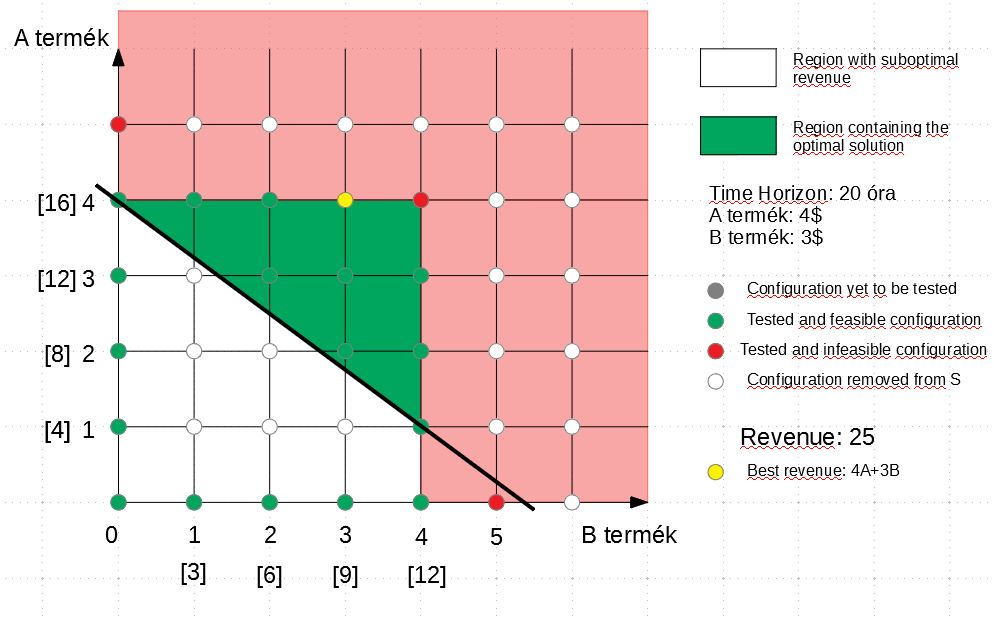
\includegraphics[scale=0.65]{throughput_szemleltetes}
\caption{Throughput maximalizálás szemléltetés}
\label{throughput_szemleltetes}
\end{center}
\end{figure}
Az algoritmus először végighalad a tengelyek mentén, vagyis az egyik termék batch mérete 0 lesz, a másik pedig növekszik. Ezt addig folytatja amíg megtalálja az első nem megvalósítható, azaz infeasible konfigurációt. Ezt követően megteszi ezt a másik tengelyen is. Így kap egy jelenleg maximális jövedelmet. Az utolsó még feasible batch méreteknél nagyobb batch mérteket már nem kell vizsgálni, hiszen azokat a megadott időhorizonton belül nem lehet megvalósítani. A képen látható feladatban ez 16 volt. A két tengelyen lévő 16 értékhez tartozó batch méretet összeköti egy vonallal. Jelenlegi példában a B termékhez tartozó 16-os érték nem egész batch mérethet tartozik, a legközelebbi a 15-tel rendelkező, ami infeasible már. A behúzott vonal alatt azok a konfigurációk szerepelnek, amelyek jövedelme nem éri ez a jelenlegi maximumot, így ezek nem a lehető legjobb megoldást adják meg. Ezek tesztelésére már nem kell időt fordítani. Az algoritmus addig folytatja a futást, amíg a halmaz, amely a konfigurációkat tartalmazza ki nem ürül. Ha nem talált megvalósítható konfigurációt, akkor az adott problémát a megadott időhorizontot belül nem lehet megoldani. Ellenkező esetben az algoritmus megadja az elérhető legnagyobb profitot, és a konfigurációt, amellyel ez elérhető. A példafeladatban a maximálisan elérhető jövedelem 25. Ezt négy darab A termék és 3 darab B termék legyártásával lehet elérni.